\documentclass[12pt, a4paper, oneside]{article}

\usepackage[brazil]{babel}
\usepackage[utf8]{inputenc}
\usepackage[T1]{fontenc}
\usepackage{graphicx}
\usepackage{url}
\usepackage{array}
\usepackage{times}
\usepackage{setspace}
\usepackage{color}
\usepackage{booktabs}
\usepackage{rotating}


\usepackage[square,numbers]{natbib}

\renewcommand*\thesection{\arabic{section}}

%\hyphenation{}

\begin{document}


\title{\textbf{Relatório do Trabalho Prático 1}\\
	\normalsize{Sistemas de Recomendação -- 2014.2}
}

\author{
    \textbf{Aécio Solano Rodrigues Santos}\\ 
    \small{\texttt{aeciosantos@dcc.ufmg.br}}\\
    \and
    \textbf{\small{Universidade Federal de Minas Gerais}}\\
    \small{Departamento de Ciência da Computação}\\
    \small{Belo Horizonte, Brasil}
}

\date{}

\maketitle

%\onehalfspacing

%------------------------------------------------------------------------------

\section{Introdução}
\label{sec:introducao}

Sistemas de Recomendação é uma área de pesquisa que está em rápido desenvolvimento na academia e na indústria. Filtragem Colaborativa é uma das técnicas clássicas utilizados por sistemas de recomendação para gerar recomendações de item personalizadas para cada usuário.

Este trabalho tem como objetivo descrever a implementação e avaliaç\~ao de um algoritmo clássico de filtragem colaborativa baseada em usuário (\textit{User-User Colaborative Filtering}). O algoritmo foi implementado usando linguagem Java 8.

O algoritmo foi avaliado usando a base de dados Movie Lens 100k. Os experimentos apresentados mostram a influência da quantidade de usuários similares utilizados para estimar o rating que um usuário daria para um determinado item da coleção de dados. É feito ainda uma comparação entre o algoritmo de filtragem colaborativa baseada em usuário com um algoritmo não personalizado simples, que estima o rating usando apenas a média dos ratings de todos os usuários da coleção. Os resultados mostram uma melhora da acurácia na predição dos ratings da abordagem personalizada de acordo com a métrica RMSE (\textit{Root Mean Square Error}). %É apresentado ainda, uma variação simples na fórmula da correlação de Pearson que melhora a acurácia do algoritmo em termos da métrica RMSE (\textit{Root Mean Square Error}).

O restante do trabalho está organizado da seguinte forma. A descrição do algoritmo implementado é apresentado na seç\~ao \ref{sec:algoritmo}. A base de dados utilizada é descrita na seç\~ao \ref{sec:dataset}. Os experimentos realizados e resultados serão apresentados na seção \ref{sec:experimentos}. Por fim, na seç\~ao \ref{sec:conclusao} constar\'a as conclus\~oes e consideraç\~oes finais.


%------------------------------------------------------------------------------

\section{Algoritmo}
\label{sec:algoritmo}
\input{algoritmo}
Esta seção apresenta uma breve descrição do algoritmo de filtragem colaborativa
baseada em usuário utilizado para fazer a predição de ratings.
A premissa básica de métodos de recomendação baseados em filtragem colaborativa é 
que as pessoas tem preferências similares, ou seja, a opinião de outros usuários pode ser
agregada de forma a prover predições das preferencias do usuário para que ser quer
fazer uma recomendação.

\subsection{User-User Colaborative Filtering (UUCF)}
\label{sec:user-to-user}
% intro
Filtragem colaborativa baseada em usuário (UUCF) foi o primeiro método de 
filtragem colaborativa automatizado proposto na literatura\cite{ekstrand2011collaborative}. O algoritmo foi proposto por Resnick et al. em 1994 como um recomendador de artigos no projeto GroupLens Usenet \cite{resnick1994grouplens}.

% perfil do usuário, matriz de ratings
O primeiro passo do algoritmo UUCF é obter um perfil do usuário. Uma forma de 
representar o perfil do usuário é usando uma matriz de ratings em que cada linha 
representa um usuário, cada coluna representa um item. O valor da célula da interseção
entre uma linha $i$ e uma coluna $j$ representa o rating do usuário $i$ no item $j$.
A ausência do valor indica que o item não foi avaliado pelo usuário.

% similidade de usuário
O segundo passo é computar a similaridade entre usuários e encontrar para cada usuário $u$,
os $k$ usuários mais semelhantes ao usuário $u$. Existem várias métricas 
para computar a similaridade entre usuários como por exemplo a correlação de pearson
e similaridade do cosseno.

% similaridade de pearson
Neste trabalho foi utilizada como similaridade a correlação de pearson que é dada por:
$$sim(a,b) = \frac{\sum\limits_{p \in P}(r_{a,p}-\bar{r_a})(r_{b,p}-\bar{r_b})}{\sqrt{\sum\limits_{p \in P}(r_{a,p}-\bar{r_a})^2\sum\limits_{p \in P}(r_{b,p}-\bar{r_b})^2}}$$

onde $x$ e $y$ são usuários, $P$ é o conjunto de itens que foram avaliados por $x$ e $y$, $r_{a,p}$ é o rating que o usuário $x$ deu ao item $p$ e $\bar{r_a}$ é a média de ratings do usuário $a$ em todos os itens.
Para os usuários que o valor da similaridade de pearson é indefinido, considerou-se a similaridade igual a zero.

O último passo é calcular uma predição de rating que o usuário daria para os itens que ele ainda não avaliou. A predição de um item $i$ é calculada pela média ponderada dos ratings que os $k$ usuários mais similares deram para o item $i$, ou seja:

$$ pred(u, i) = \bar{r_u} +  \frac{ \sum\limits_{u^\prime \in U} sim(u,u^\prime)(r_{u^\prime, i} - \bar{r_{u^\prime}}) }{ \sum_{u^\prime \in U} |sim(u,u^\prime)| } $$

\subsection{Análise de Complexidade do Algoritmo UUCF}

Apesar de ser um algoritmo intuitivo, a complexidade do algoritmo pode ser um problema para computação em bases de dados reais. A cálculo da similaridade entre dois usuários (usando a Correlação de Pearson) tem complexidade $O(N)$, sendo $N$ o número de itens da matriz. Portanto, a computação da similaridade de um usuário com os demais é da ordem de $O(MN)$, sendo $M$ a quantidade de usuários. Como a similaridade deve ser computada para todos os usuários da matriz, o cálculo de todas as similaridades par-a-par é $O(M^{2}N)$.

%\pagebreak

%------------------------------------------------------------------------------
\section{Dataset}
\label{sec:dataset}
Para avaliar o algoritmo foi utilizada a base dados MovieLens 100k. Esta base contém 100,000 ratings
com escala de 1 a 5 dados por 943 usuários para 1682 filmes. Cada usuário avaliou pelo menos 20 filmes.
Além disso, a base contém informações demográficas simples sobre os usuários, porém essas informações 
não foram utilizadas neste trabalho. O Dataset está publicamente disponível em \texttt{http://grouplens.org/datasets/movielens/}.
%------------------------------------------------------------------------------
\section{Experimentos}
\label{sec:experimentos}
O primeiro experimento realizado teve o objetivo de identificar como a quantidade $k$ de usuários mais similares
influência a eficácia do algoritmo. Nesse experimento utilizou-se a o arquivo \texttt{ua.base} para o
treinamento do algoritmo, e o arquivo \texttt{ua.test} para computar a acurácia.
A acurácia é foi medida utilizando a métrica RMSE (root mean squared error), dada por:
$$ RMSE = \sqrt{ \frac{1}{n}\sum_{i=1}^n(\hat{Y_i} - Y_i)^2} $$
onde $\hat{Y_i}$ é o rating calculado pelo algoritmo e $Y_i$ é o rating real que o usuário deu para o item $i$.

A Figura \ref{fig:uucf-rmse-k} mostra o resultado da variação do valor de número de usuários similares. A medida que o número de usuários aumenta, a acurácia melhora. Porém, para valores a partir de 50 a acurácia diminui. Isso pode ocorrer devido a introdução de ruídos a medida que a quantidade de usuários aumenta muito.
\pagebreak
Na coleção Movie Lens 100k, 50 se mostrou o número de usuário que dá melhores resultados, portanto esse valor foi escolhido para comparar com um baseline não personalizado como descrito a seguir.

\begin{figure}[!th]
\centering
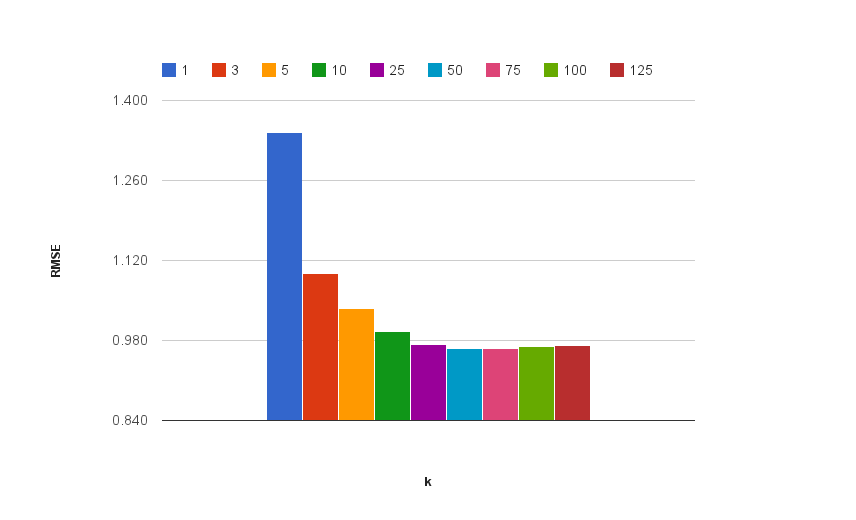
\includegraphics[scale=.45]{img/uucf-rmse-k.png} 
\caption{Influência de valores de $k$ na acurácia de predições}
\label{fig:uucf-rmse-k}
\end{figure}

A tabela \ref{tab:rmse} mostra um comparativo entre a acurácia do algoritmo UUCF com $k=50$ e um algoritmo que prediz o rating baseado no rating médio de todos itens, ou seja:
$$ pred(u, i) = \frac{1}{|R_i|} \sum\limits_{r \in R_i} r $$
onde $R_i$ é o conjunto de todos os ratings dados ao item $i$.

\begin{table}[!ht]
\centering
\begin{tabular}{|c|c|}
\hline
\textbf{Algoritmo}   & \textbf{RMSE} \\ \hline
UUCF k=50            & 0.967 \\ \hline
Rating médio do item & 1.042 \\ \hline
\end{tabular}
\caption{Acurácia de algoritmos de acordo com métrica RMSE}
\label{tab:rmse}
\end{table}


Devido a capacidade de personalização dos ratings para cada usuário, o algoritmo UUCF consegue melhores resultados que um algoritmo não personalizado que leva em conta somente qualidade média de um item.

%------------------------------------------------------------------------------
\section{Conclusão}
\label{sec:conclusao}
Nesse trabalho, descrevemos o algoritmo de filtragem colaborativa baseado em usuário (User-User Colaborative Filtering) e apresentamos um estudo sobre a influência da quantidade de usuários similares na acurácia do algoritmo. Foi mostrado que o algoritmo consegue melhorias comparado a um algoritmo não personalizado por levar em conta as preferências de cada usuário ao calcular os ratings. Porém, dado a alta complexidade de execução no pior caso do algoritmo, pode ser inviável a execução do algoritmo em grandes bases de dados com milhões de usuários e itens. Alguns passos do algoritmo podem ser computados offline, como a matriz de similaridade entre usuários e média de ratings de cada usuário, para diminuir tempo de resposta da recomendação online. Porém, mesmo assim ainda pode ser necessário recorrer ao uso de outros algoritmos de recomendação mais eficientes.
%------------------------------------------------------------------------------

\bibliography{tp01}
\bibliographystyle{plain}

\end{document}
